\documentclass[]{article}
\usepackage[spanish]{babel}
\usepackage{graphicx}

%opening
\title{
\includegraphics[width=4cm]{UTN_logo.jpg}\\[2cm]Trabajo Practico 1 - Energía, Potencia, Eficiencia \textbf{Física II}}

\author{
	Díaz, Santiago Alberto\\
	\texttt{Legajo: 55384}
	\and
	Rover, Natalio\\
	\texttt{Legajo: 404591}
	\and
	Piccinini, Gonzalo\\
	\texttt{Legajo: 413776}
	\and
	Sánchez, Julián Alejandro\\
	\texttt{Legajo: 413544}
}

\begin{document}

\maketitle

\newpage
\section{Resumen teórico básico}

\subsection{Temperatura y ley cero de la Termodinámica}
\begin{flushleft}
	\textbf{Ley cero de la Termodinámica}: Si dos objetos A y B están por separado en equilibrio térmico con un tercer objeto C, se dice que A y B están en equilibrio térmico entre sí.
\end{flushleft}
\begin{flushleft}
	\textbf{Temperatura}: Propiedad que determina si un objeto está en equilibrio térmico con otros objetos. Dos objetos en equilibrio térmico uno con el otro están a la misma temperatura.
\end{flushleft}


\subsection{Calor y Energía}
\begin{flushleft}
	\textbf{Calor}: El calor es la transferencia de energía a través de la frontera de un sistema debido a una diferencia de temperatura entre el sistema y el ambiente.
\end{flushleft}

\begin{flushleft}
	\textbf{Energía interna}: Es toda la energía de un sistema asociada a componentes microscópicos(átomos y moléculas).
\end{flushleft}

\subsection{Calor especifico}
\begin{flushleft}
	\textbf{Capacidad térmica}: Cantidad de energía necesaria para elevar la temperatura de un muestra en 1°C, dicha energía Q produce un cambio de temperatura $\bigtriangleup T$. 
	
	\begin{center}
		(1) $Q = C \cdot \bigtriangleup T$
	\end{center}
\end{flushleft}

\begin{flushleft}
	\textbf{Calor específico}: Es la capacidad térmica por unidad de masa.
	\begin{center}
		(2) $c = \frac{Q}{m \cdot \bigtriangleup T}$
	\end{center}
	
	\begin{flushleft}
		Donde: \\
		\textbf{m}: Masa de una muestra de sustancia. \\
		\textbf{Q}: Energía transferida a la sustancia \textbf{m}. \\
		\textbf{$\bigtriangleup T$}: Cambio de temperatura. \\
	\end{flushleft}
	
	\begin{flushleft}
		A partir de está definición se puede relacionar la energía transferida entre una sustancia de masa \textbf{m} y sus alrededores con un cambio de temperatura $\bigtriangleup T$.
		
		\begin{center}
			(3) $Q = m \cdot c \cdot \bigtriangleup T$
		\end{center}
	\end{flushleft}
\end{flushleft}

\subsection{Potencia}
Potencia se define como la relación que existe entra la cantidad de energía transferida desde un sistema con el tiempo requerido para realizarse dicha transferencia.

\begin{center}
	(4) $P = \frac{E}{t}$
\end{center}
\subsection{Eficiencia}
\begin{flushleft}
	La eficiencia energética es la relación entre la cantidad de energía útil que se obtiene de un sistema y la cantidad de energía que se ha invertido para lograrlo. En otras palabras, mide cuán eficazmente se utiliza la energía para realizar una tarea o producir un servicio. Un sistema es más eficiente energéticamente cuando produce más trabajo útil con menos consumo de energía.
\end{flushleft}
\begin{center}
	(5) $\eta = \frac{\epsilon_{util}}{\epsilon_{total}}$
\end{center}

\section{Descripción de la experiencia}
\begin{flushleft}
	Este informe describe una experiencia cuya finalidad es calcular de forma experimental el \textbf{rendimiento} energético de un sistema de calentamiento de agua al punto de ebullición (100°C), ya sea suministrando energía por medio de la red electrica (pava electrica) o suministrando calor por fuego o por el horno de la cocina.
\end{flushleft}

\subsection{Primera experiencia - Pava eléctrica}

\begin{flushleft}
	Para la primer experiencia utilizamos una pava eléctrica marca philco
	con capacidad máxima de agua de 1.7 Litros.
\end{flushleft}
\begin{center}
	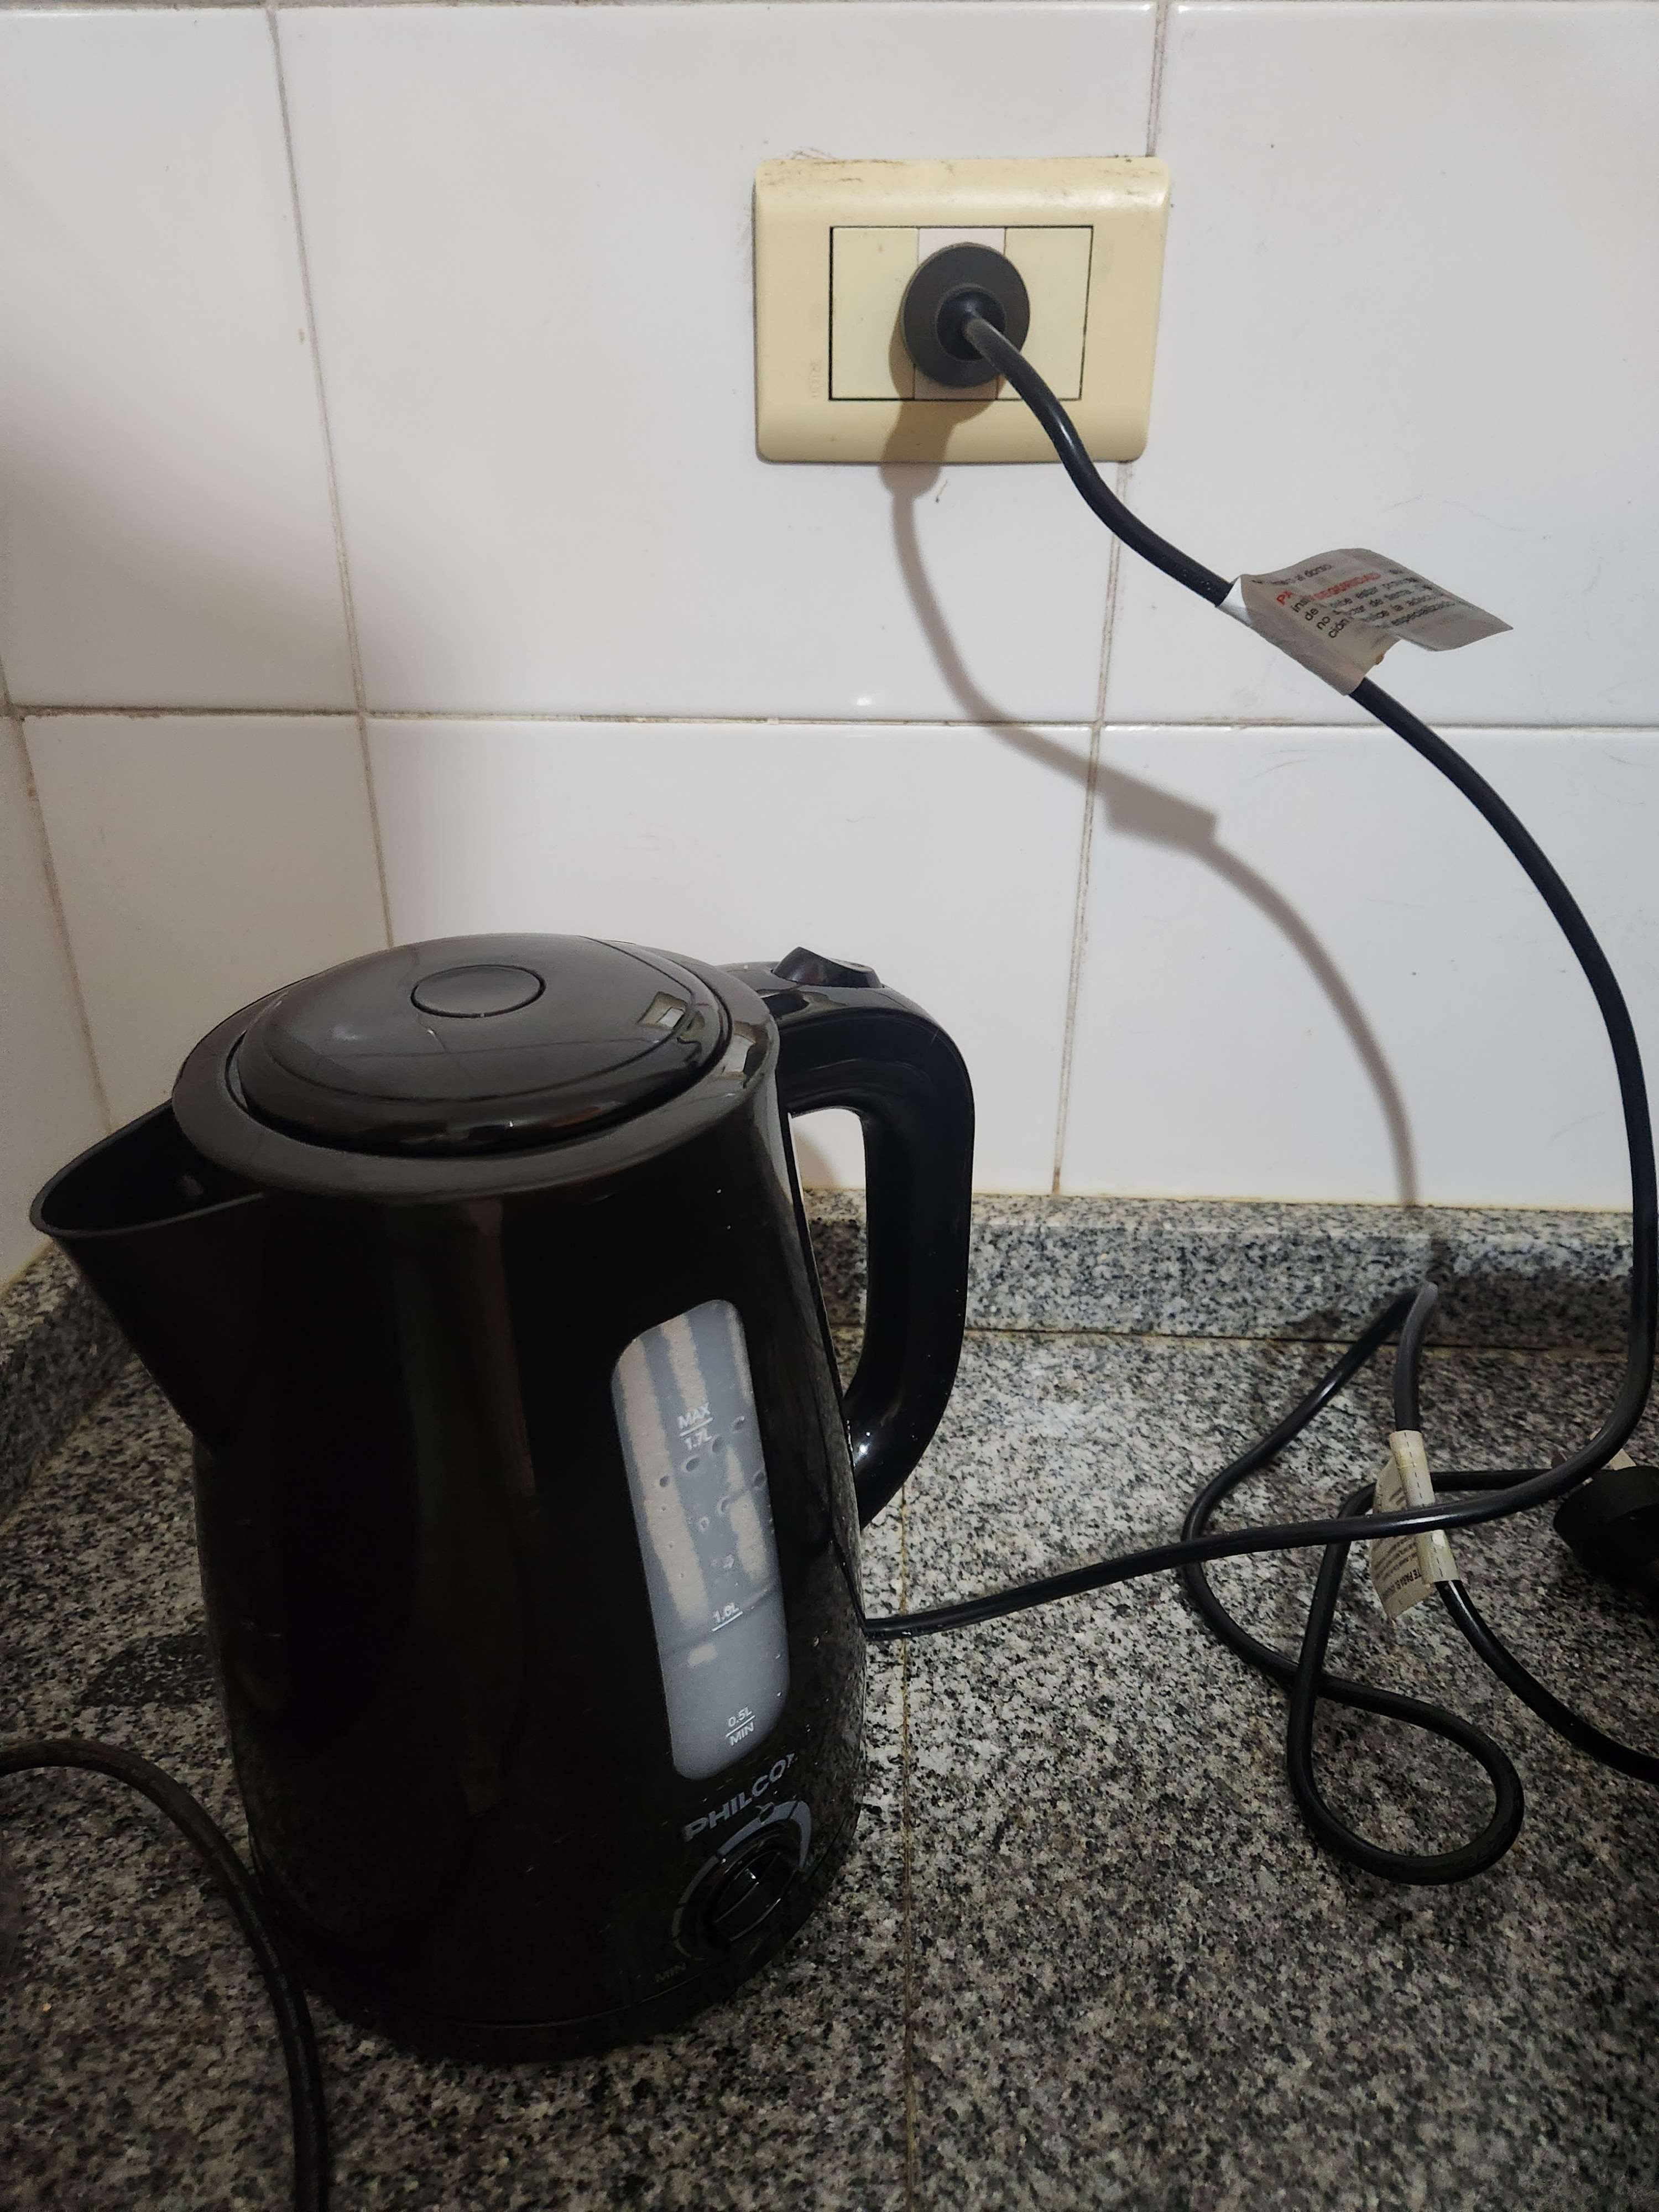
\includegraphics[width=7cm]{pava1.jpg}
\end{center}

\newpage

\begin{flushleft}
	La misma tiene una potencia de 2200 W según las especificaciones del fabricante.
\end{flushleft}
\begin{center}
	
\includegraphics[width=6cm]{pava2.jpg}
\end{center}

\begin{center}
	Como primer paso llenamos la pava con 1 litro de agua.
\end{center}
\begin{center}
	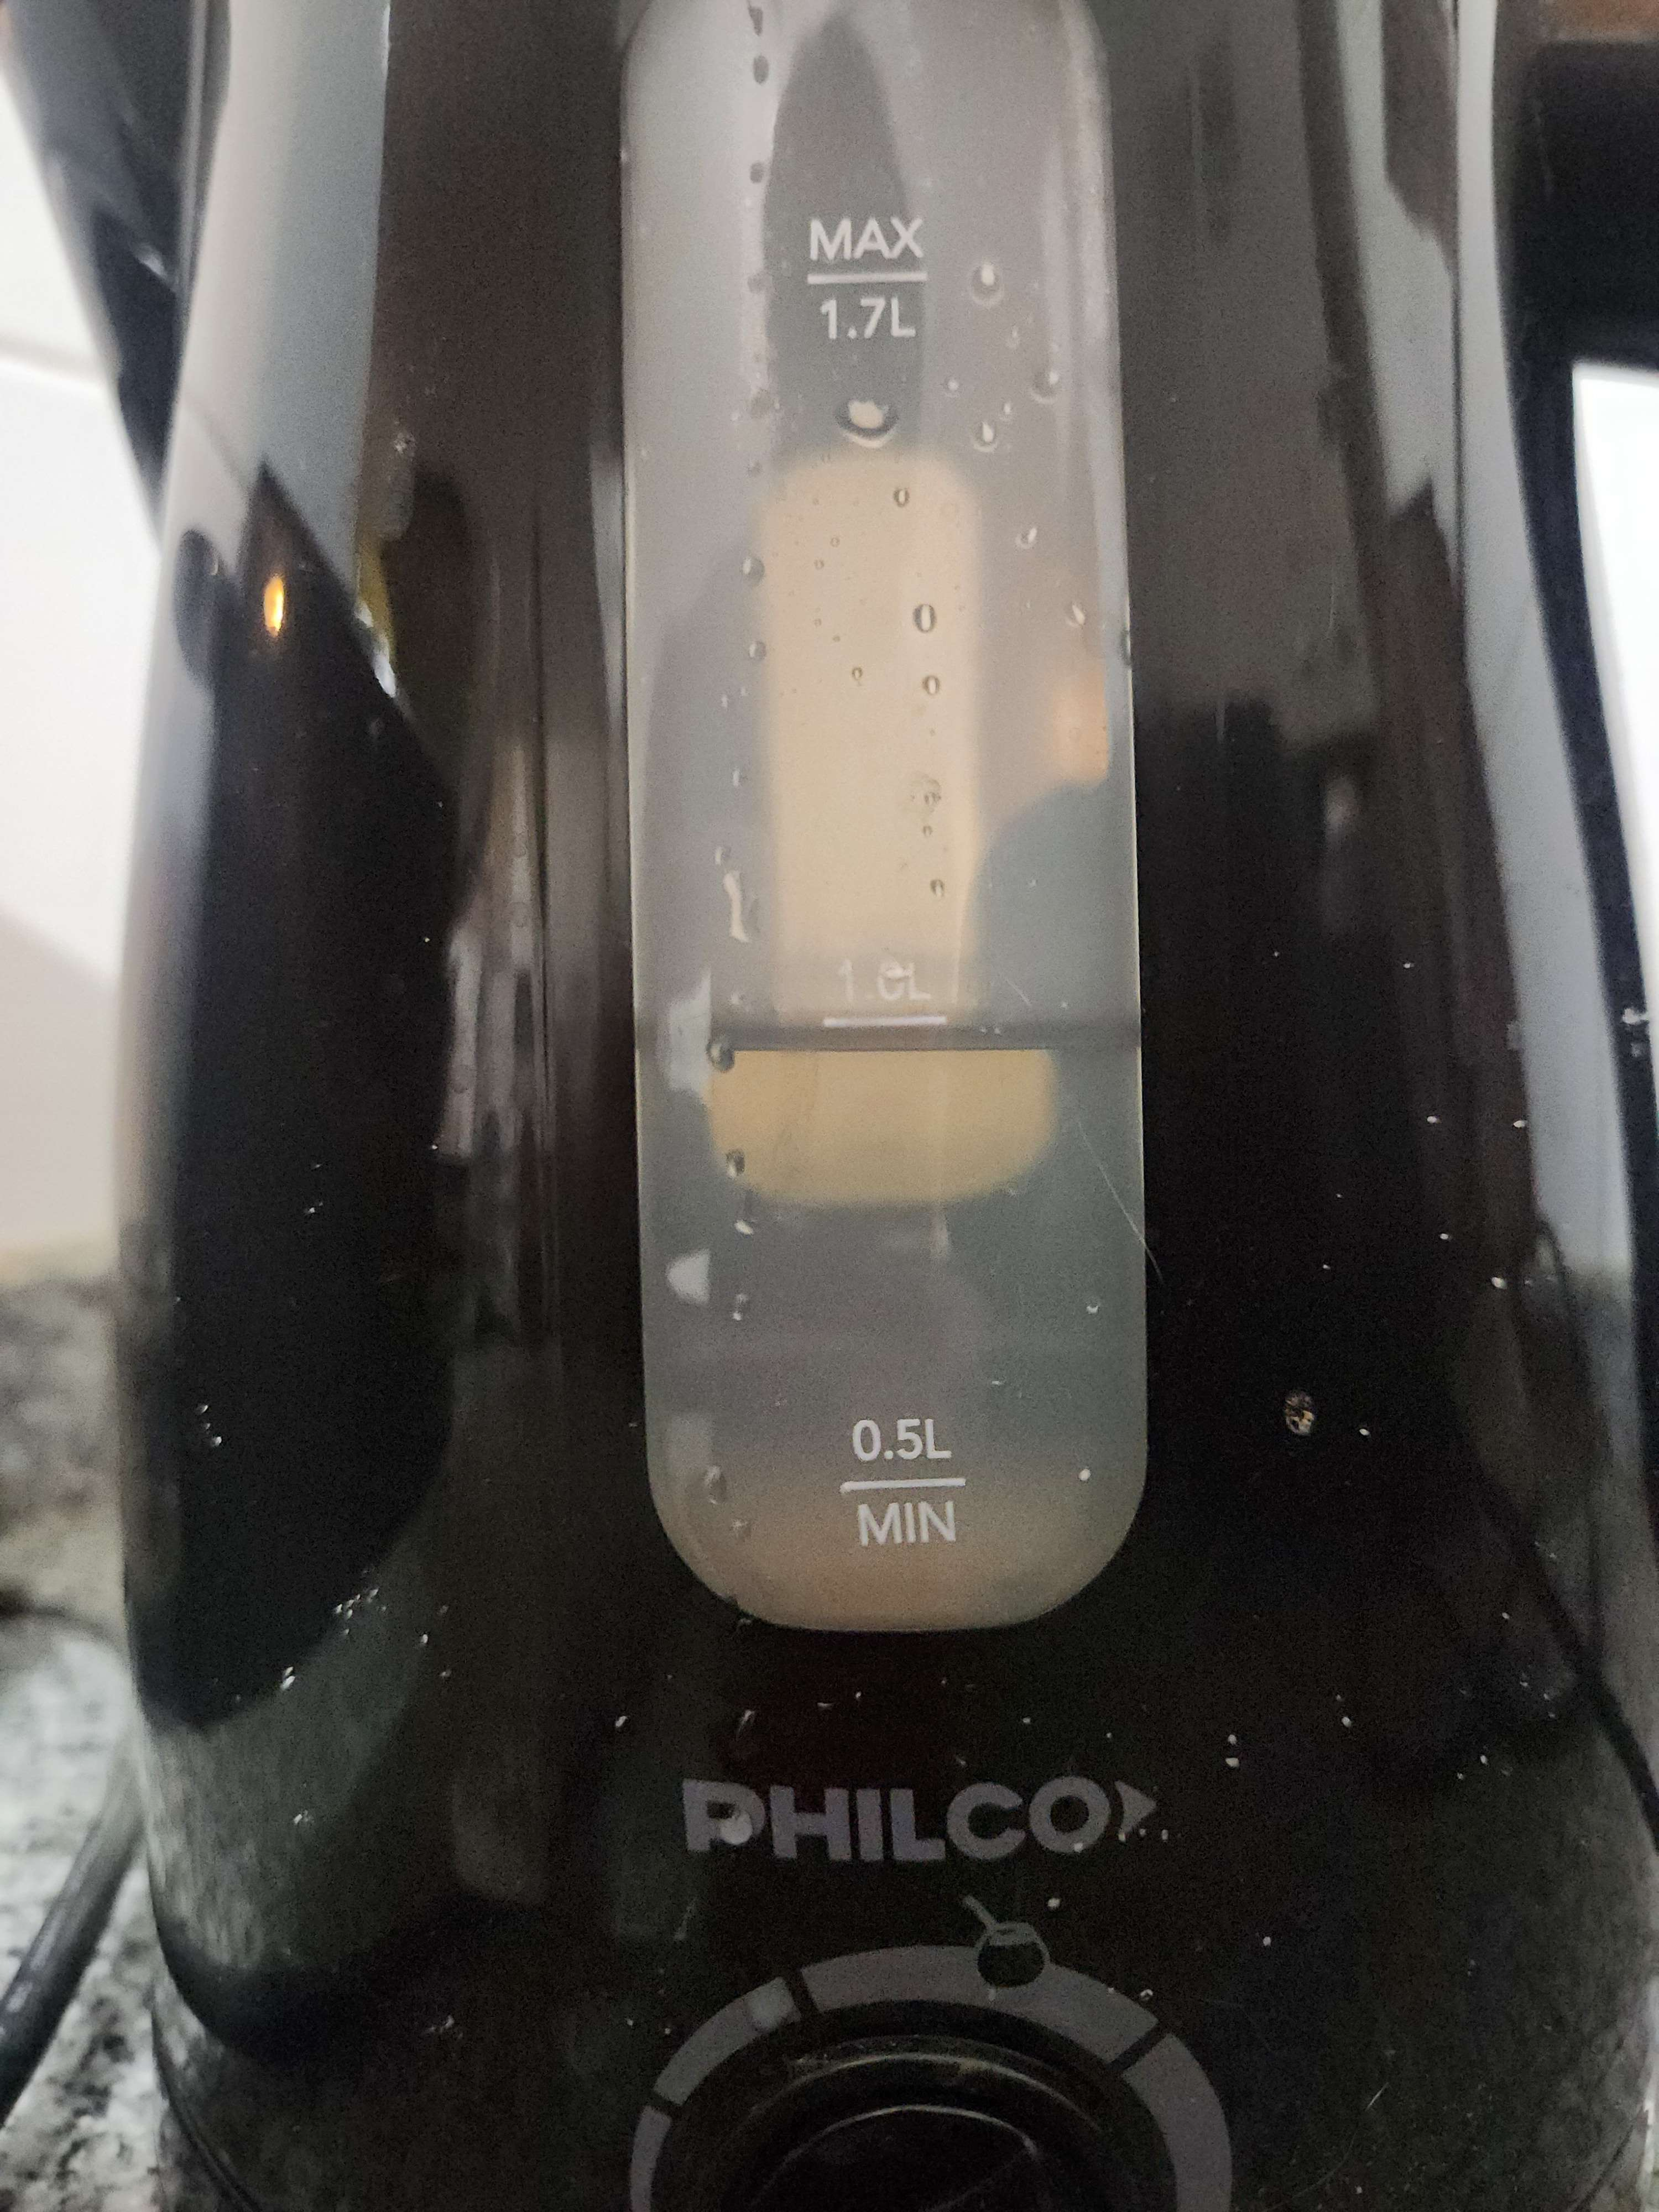
\includegraphics[width=6cm]{pava3.jpg}
\end{center}

\newpage

\begin{center}
	Luego llevamos la pava al balcón para que tome la temperatura ambiente la cual usaremos como temperatura inicial la cual tomaremos del pronostico del día de la experiencia.
\end{center}
\begin{center}
	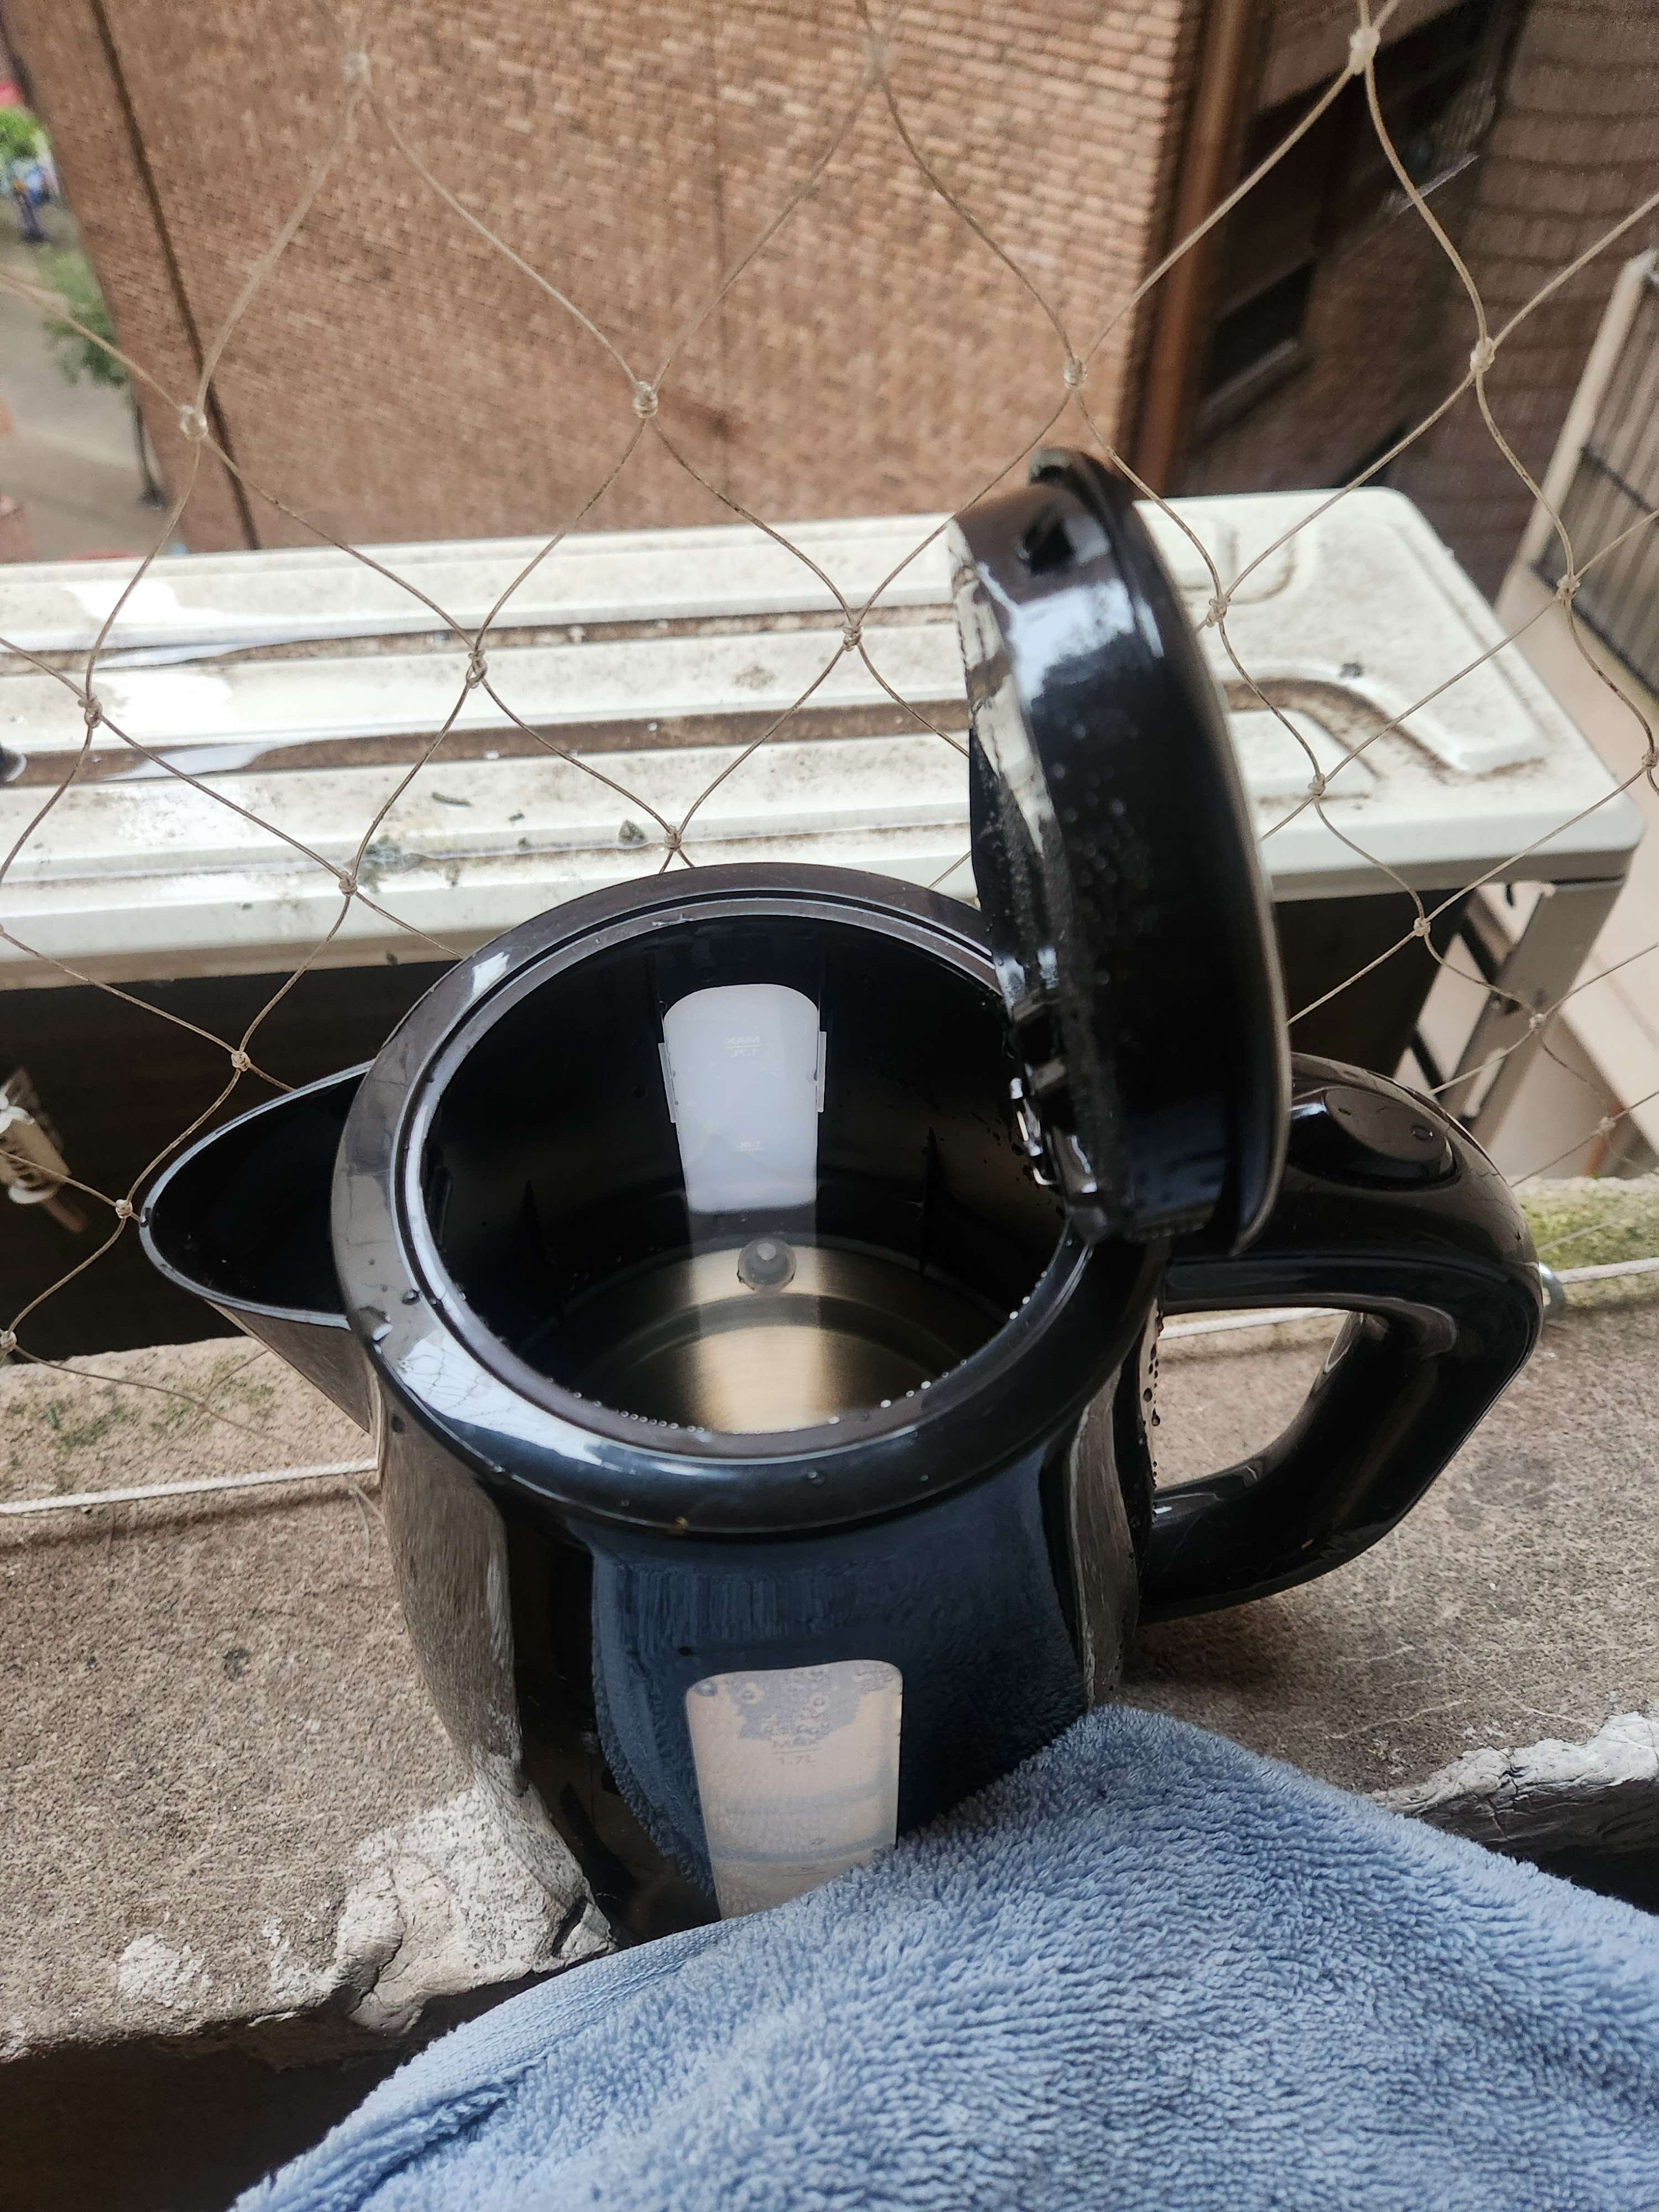
\includegraphics[width=6cm]{pava4.jpg}
\end{center}
\begin{center}
	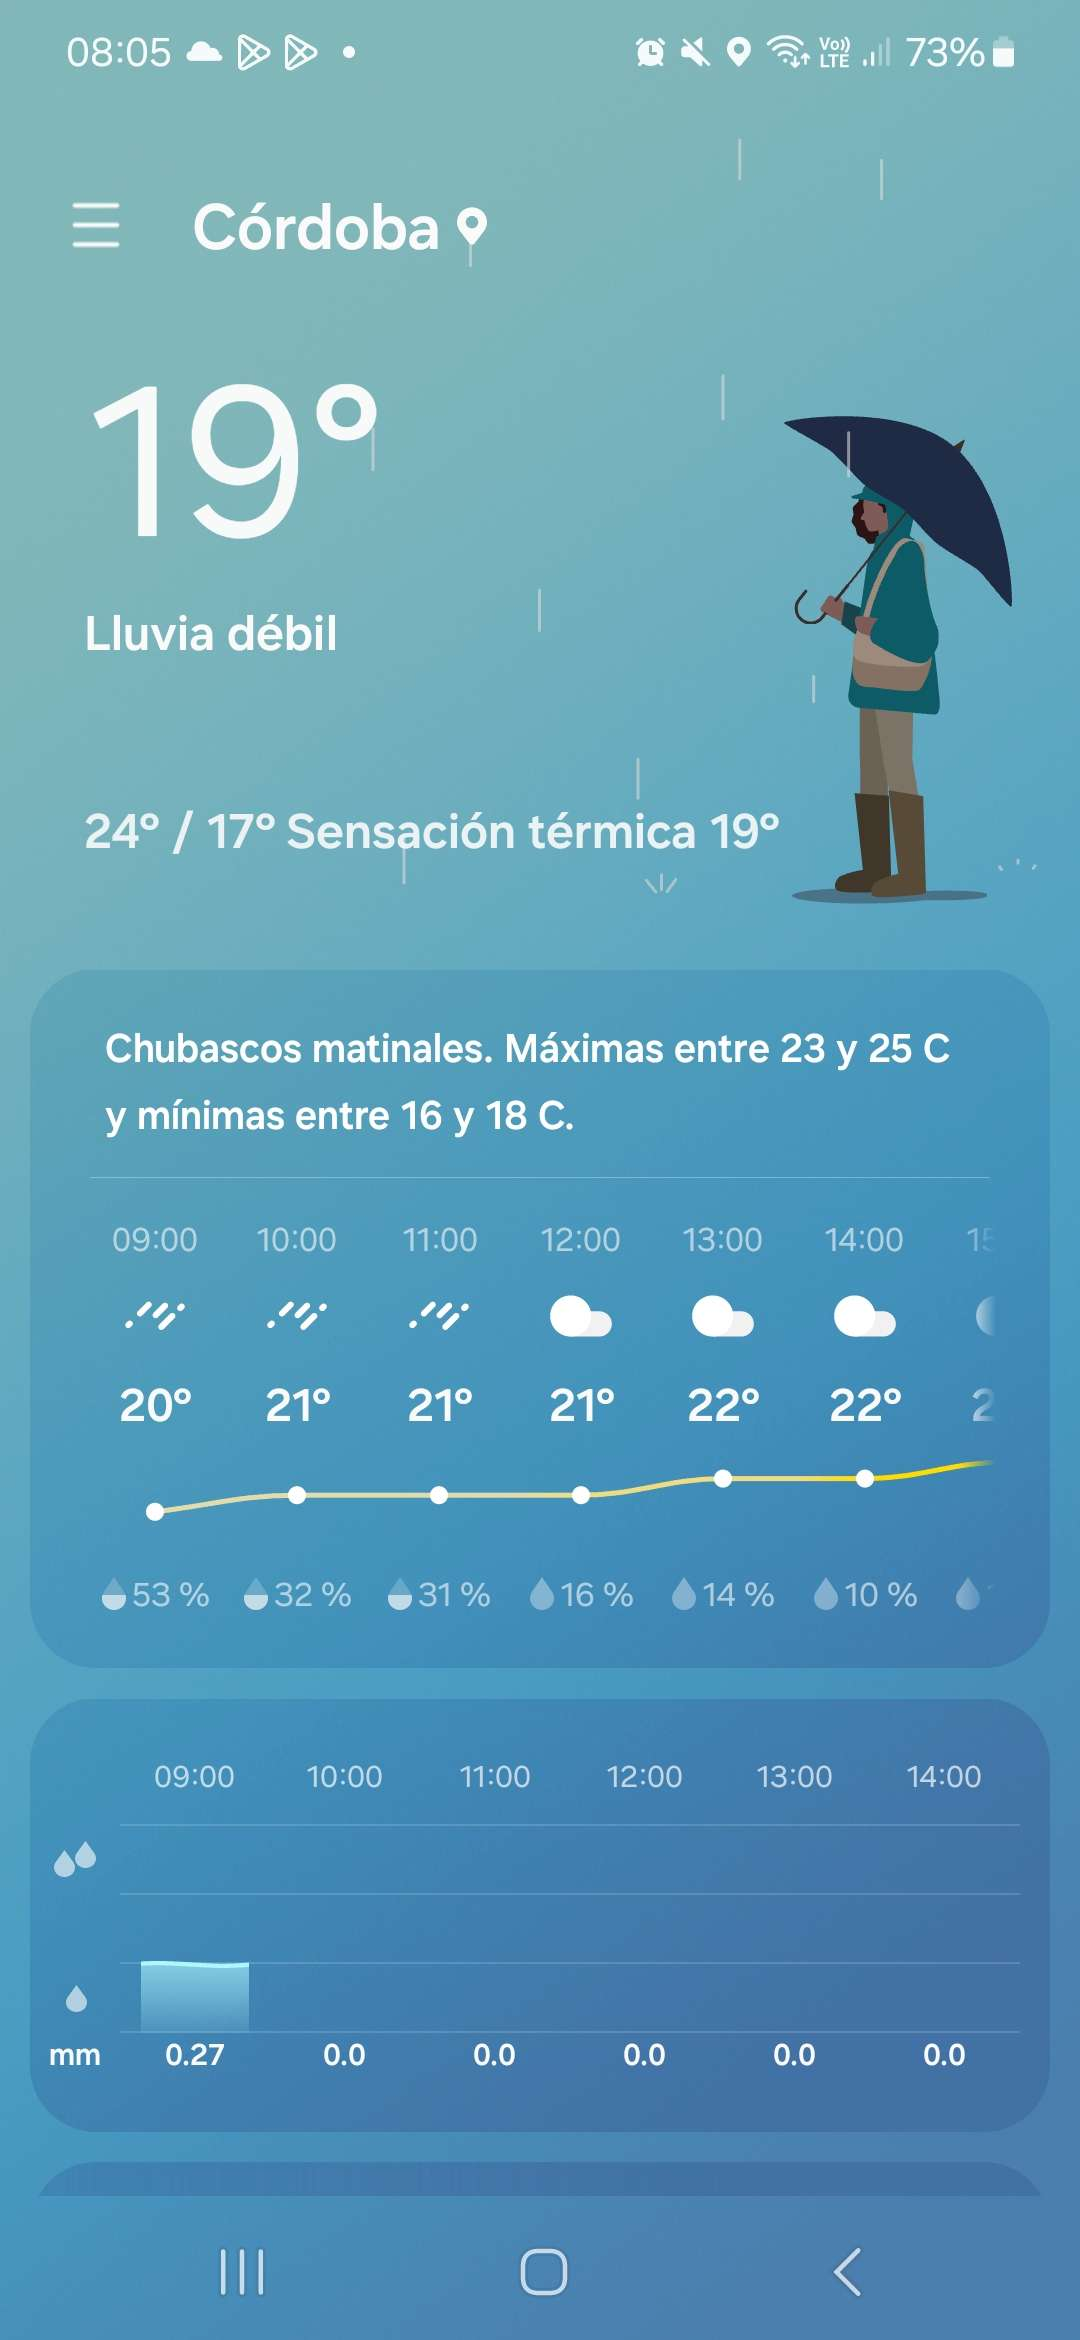
\includegraphics[width=4cm]{pava5.jpg}
\end{center}

\newpage

\begin{center}
	A continuación enchufamos la pava eléctrica y en el momento que la encendemos empezamos a cronometrar el tiempo en que tarda en hervir, detenemos el cronometro en el momento que el botón salta solo.
\end{center}
\begin{center}
	
\includegraphics[width=4cm]{pava6.jpg}
\end{center}

\section{Cálculos}
\subsection{Primera experiencia - Pava eléctrica}
\begin{flushleft}
	En base a la experiencia realizada podemos obtener valores iniciales de tiempo y temperatura necesarios para calcular el rendimiento.
\end{flushleft}

\begin{itemize}
	\item \textbf{Temperatura inicial} $T_{i} = 19$ °C
	\item \textbf{Temperatura final o equilibrio} $T_{f} = 100$ °C
	\item \textbf{Tiempo que tardo en calentarse}: 2 minutos con 44 segundos.
	\item \textbf{Potencia de la pava} $P = 2200$ W
	\item \textbf{Calor especifico del agua} $C_{e} = 4190 \frac{J}{KgK}$ 
\end{itemize}

\begin{flushleft}
	Como primer paso calculamos la energía suministrada por la red eléctrica la cual necesitamos para obtener el rendimiento. Por medio de la experiencia cronometramos un tiempo de 2 minutos y 44 segundos, que en total serian unos 164 segundos.
	
	\begin{center}
		$t = 164$ s
	\end{center}
	
	Por medio de la formula (4) obtenemos la energía suministrada por el enchufe.
	
	\begin{center}
		$P = \frac{\epsilon_{t}}{t}$
	\end{center}
	\begin{center}
		$\epsilon_{t} = P \cdot t$
	\end{center}
	\begin{center}
		$\epsilon_{t} = 2200 W \cdot 164 s$
	\end{center}
	\begin{center}
		$\epsilon_{t} = 360800$ J
	\end{center}
\end{flushleft}

\begin{flushleft}
	Ahora calculamos la energía útil que sera la que el sistema recibe de parte de la red para calentar el agua, por lo tanto está energía llega al agua en forma de calor por lo que podemos utilizar la formula (3).
	
	\begin{center}
		$Q = m \cdot C_{e} \cdot \bigtriangleup T$
	\end{center}
	
	Donde:
	\begin{itemize}
		\item \textbf{Masa de agua} $m = 1$ Kg
		\item \textbf{Calor especifico del agua} $C_{e} = 4190 \frac{J}{KgK}$ 
		\item \textbf{Cambio de temperatura}: \\
		$\Delta T = (100 - 19)$ °C = $(373 - 292)$ K = 81 K.
	\end{itemize}
	
	\begin{flushleft}
		Entonces aplicando la formula (4) utilizando los valores previamente listados obtenemos la energía útil.
	\end{flushleft}
	
	\begin{center}
		$\epsilon_{util} = m \cdot C_{e} \cdot \bigtriangleup T$
	\end{center}
	\begin{center}
		$\epsilon_{util} = 1 Kg \cdot 4190 \frac{J}{KgK} \cdot 81 K$
	\end{center}
	
	\begin{center}
		$\epsilon_{util} = 339390$ J
	\end{center}
\end{flushleft}

\begin{flushleft}
	Ahora ya tenemos todos los datos para calcular el rendimiento energético usando la formula (5).
	
	\begin{center}
		$\eta = \frac{\epsilon_{util}}{\epsilon_{total}}$
	\end{center}
	\begin{center}
		$\eta = \frac{339390 J}{360800J}$
	\end{center}
	\begin{center}
		$\eta = 0.94$
	\end{center}
	
	Multiplicando por 100 obtenemos el rendimiento en porcentaje el cual es del 94\%
\end{flushleft}

\end{document}
